\documentclass{whiteboard}
\begin{document}
\begin{frame}[plain,t]
\bbcover{Grafos}{Algoritmo de Kruskall}{Prof. Edson Alves}{Faculdade UnB Gama}

\end{frame}
\begin{frame}[plain,t]
\begin{tikzpicture}
\node[draw,opacity=0] at (0, 0) {x};
\node[draw,opacity=0] at (14, 8) {x};

	\node[anchor=west] (title) at (0.0, 7.0) { \Large \bbbold{Proponente} };

	\node[] (floyd) at (7.0, 4.0) { \includegraphics[scale=0.4]{figs/kruskal.jpeg} };

	\node[] (fname) at (7.0, 1.0) { \bbbold{Joseph Bernard Kruskall, Jr.} };

	\node[] (fdate) at (7.0, 0.5) { \bbtext{(1962)} };

\end{tikzpicture}
\end{frame}
\begin{frame}[plain,t]
\begin{tikzpicture}
\node[draw,opacity=0] at (0, 0) {x};
\node[draw,opacity=0] at (14, 8) {x};

	\node[anchor=west] (title) at (0.0, 7.0) { \Large \bbbold{Características do algoritmo de Kruskall} };
\end{tikzpicture}
\end{frame}
\begin{frame}[plain,t]
\begin{tikzpicture}
\node[draw,opacity=0] at (0, 0) {x};
\node[draw,opacity=0] at (14, 8) {x};

	\node[anchor=west] (title) at (0.0, 7.0) { \Large \bbbold{Características do algoritmo de Kruskall} };

	\node[anchor=west] (a) at (1.0, 6.0) { $\star$ \bbtext{O algoritmo de Kruskall encontra uma MST usando uma abordagem gulosa} };

\end{tikzpicture}
\end{frame}
\begin{frame}[plain,t]
\begin{tikzpicture}
\node[draw,opacity=0] at (0, 0) {x};
\node[draw,opacity=0] at (14, 8) {x};

	\node[anchor=west] (title) at (0.0, 7.0) { \Large \bbbold{Características do algoritmo de Kruskall} };

	\node[anchor=west] (a) at (1.0, 6.0) { $\star$ \bbtext{O algoritmo de Kruskall encontra uma MST usando uma abordagem gulosa} };


	\node[anchor=west] (b) at (1.0, 5.0) { $\star$ \bbtext{As arestas são ordenadas, ascendentemente, por peso} };

\end{tikzpicture}
\end{frame}
\begin{frame}[plain,t]
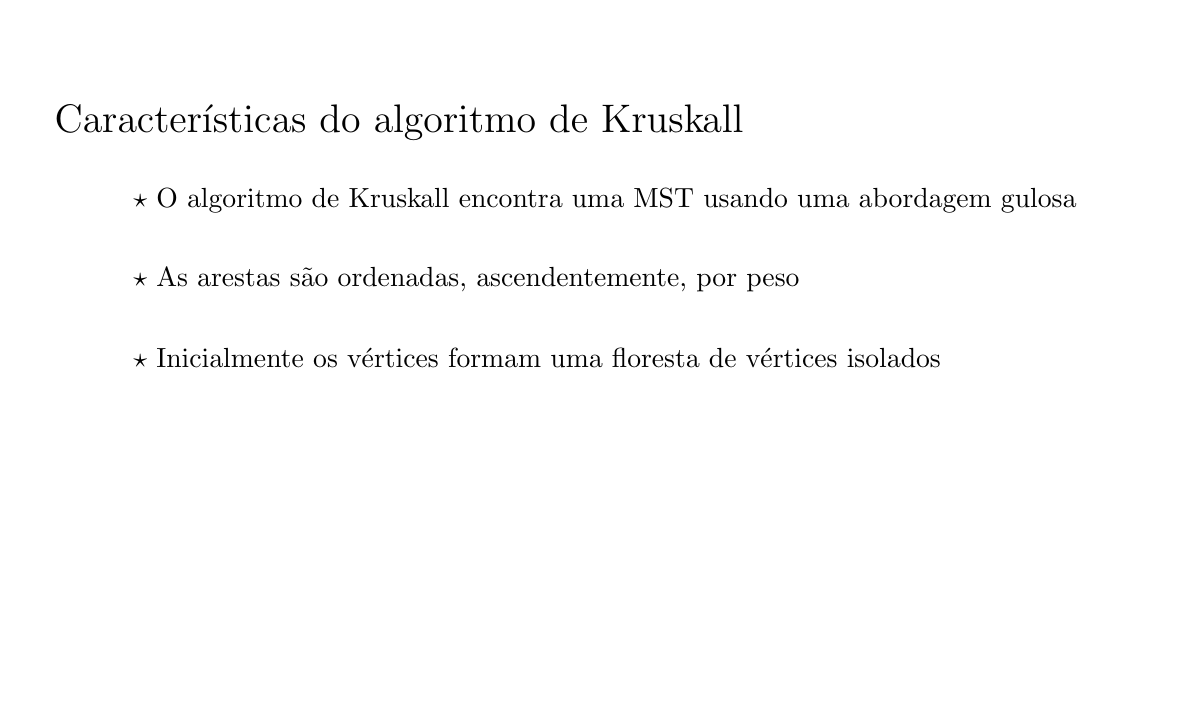
\begin{tikzpicture}
\node[draw,opacity=0] at (0, 0) {x};
\node[draw,opacity=0] at (14, 8) {x};

	\node[anchor=west] (title) at (0.0, 7.0) { \Large \bbbold{Características do algoritmo de Kruskall} };

	\node[anchor=west] (a) at (1.0, 6.0) { $\star$ \bbtext{O algoritmo de Kruskall encontra uma MST usando uma abordagem gulosa} };


	\node[anchor=west] (b) at (1.0, 5.0) { $\star$ \bbtext{As arestas são ordenadas, ascendentemente, por peso} };


	\node[anchor=west] (c) at (1.0, 4.0) { $\star$ \bbtext{Inicialmente os vértices formam uma floresta de vértices isolados} };

\end{tikzpicture}
\end{frame}
\begin{frame}[plain,t]
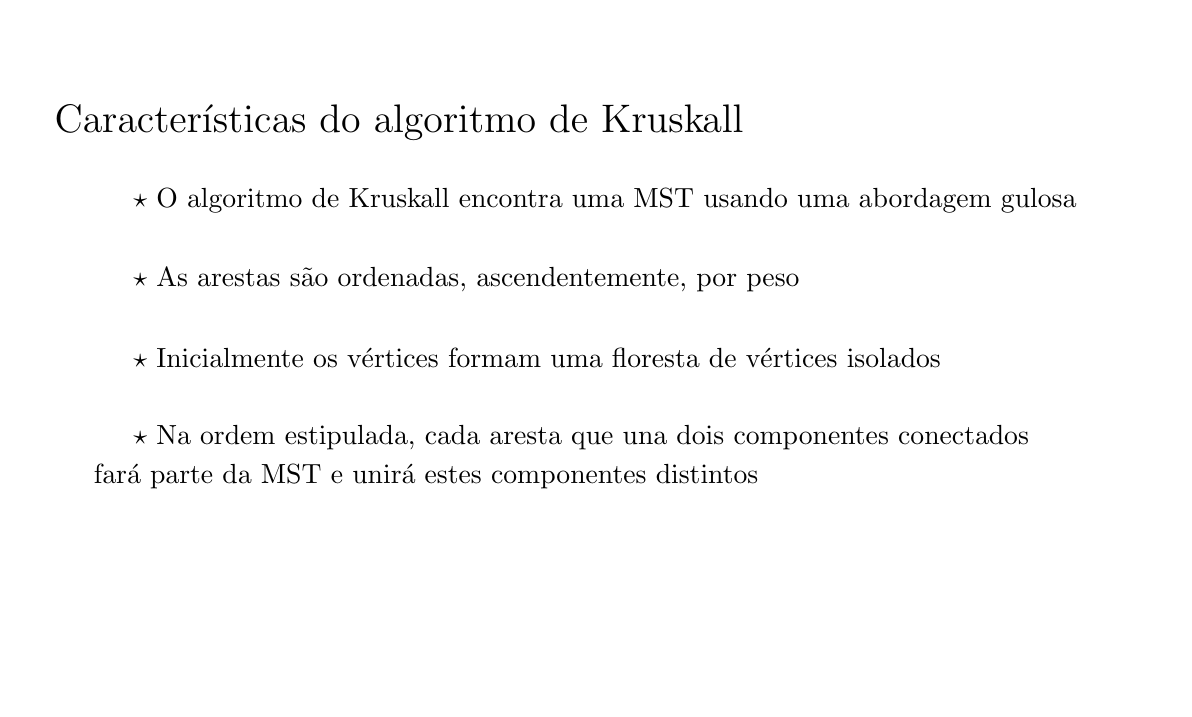
\begin{tikzpicture}
\node[draw,opacity=0] at (0, 0) {x};
\node[draw,opacity=0] at (14, 8) {x};

	\node[anchor=west] (title) at (0.0, 7.0) { \Large \bbbold{Características do algoritmo de Kruskall} };

	\node[anchor=west] (a) at (1.0, 6.0) { $\star$ \bbtext{O algoritmo de Kruskall encontra uma MST usando uma abordagem gulosa} };


	\node[anchor=west] (b) at (1.0, 5.0) { $\star$ \bbtext{As arestas são ordenadas, ascendentemente, por peso} };


	\node[anchor=west] (c) at (1.0, 4.0) { $\star$ \bbtext{Inicialmente os vértices formam uma floresta de vértices isolados} };


	\node[anchor=west] (d) at (1.0, 3.0) { $\star$ \bbtext{Na ordem estipulada, cada aresta que una dois componentes conectados} };

	\node[anchor=west] (d1) at (0.5, 2.5) { \bbtext{fará parte da MST e unirá estes componentes distintos} };


\end{tikzpicture}
\end{frame}
\begin{frame}[plain,t]
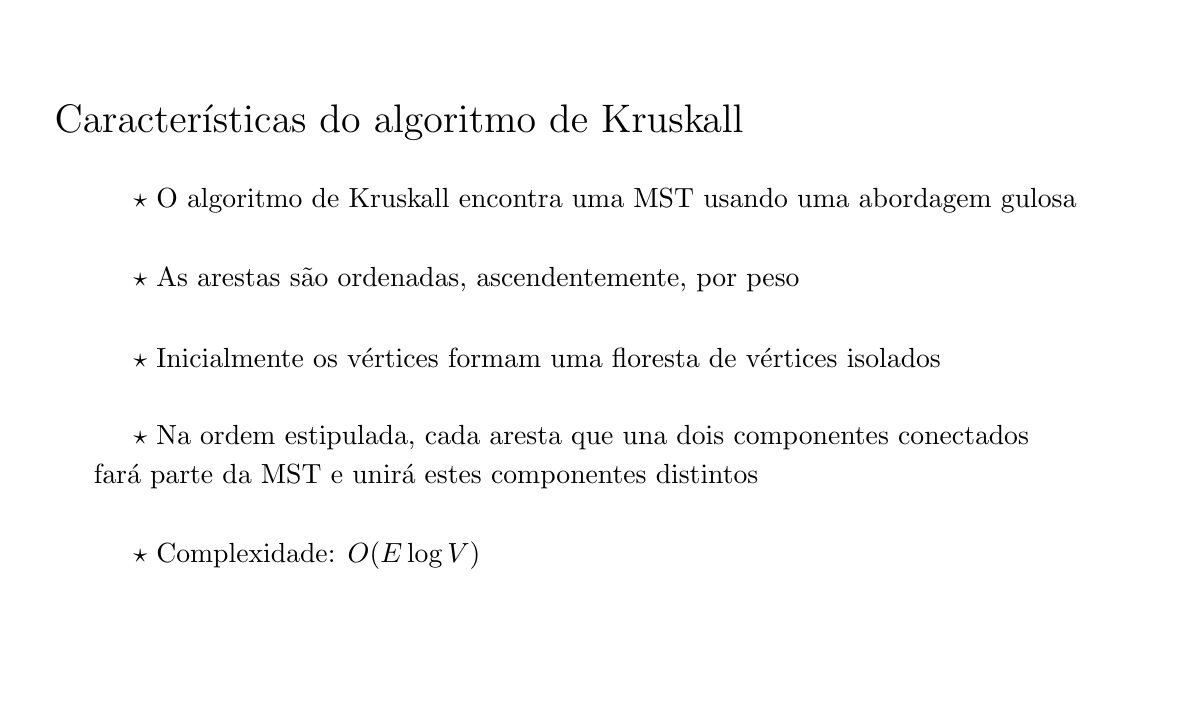
\begin{tikzpicture}
\node[draw,opacity=0] at (0, 0) {x};
\node[draw,opacity=0] at (14, 8) {x};

	\node[anchor=west] (title) at (0.0, 7.0) { \Large \bbbold{Características do algoritmo de Kruskall} };

	\node[anchor=west] (a) at (1.0, 6.0) { $\star$ \bbtext{O algoritmo de Kruskall encontra uma MST usando uma abordagem gulosa} };


	\node[anchor=west] (b) at (1.0, 5.0) { $\star$ \bbtext{As arestas são ordenadas, ascendentemente, por peso} };


	\node[anchor=west] (c) at (1.0, 4.0) { $\star$ \bbtext{Inicialmente os vértices formam uma floresta de vértices isolados} };


	\node[anchor=west] (d) at (1.0, 3.0) { $\star$ \bbtext{Na ordem estipulada, cada aresta que una dois componentes conectados} };

	\node[anchor=west] (d1) at (0.5, 2.5) { \bbtext{fará parte da MST e unirá estes componentes distintos} };



	\node[anchor=west] (e) at (1.0, 1.5) { $\star$ \bbtext{\bbbold{Complexidade}: $O(E\log V)$ } };

\end{tikzpicture}
\end{frame}
\begin{frame}[plain,t]
\begin{tikzpicture}
\node[draw,opacity=0] at (0, 0) {x};
\node[draw,opacity=0] at (14, 8) {x};

	\node[anchor=west] (title) at (0.0, 7.0) { \Large \bbbold{Pseudocódigo} };

\end{tikzpicture}
\end{frame}
\begin{frame}[plain,t]
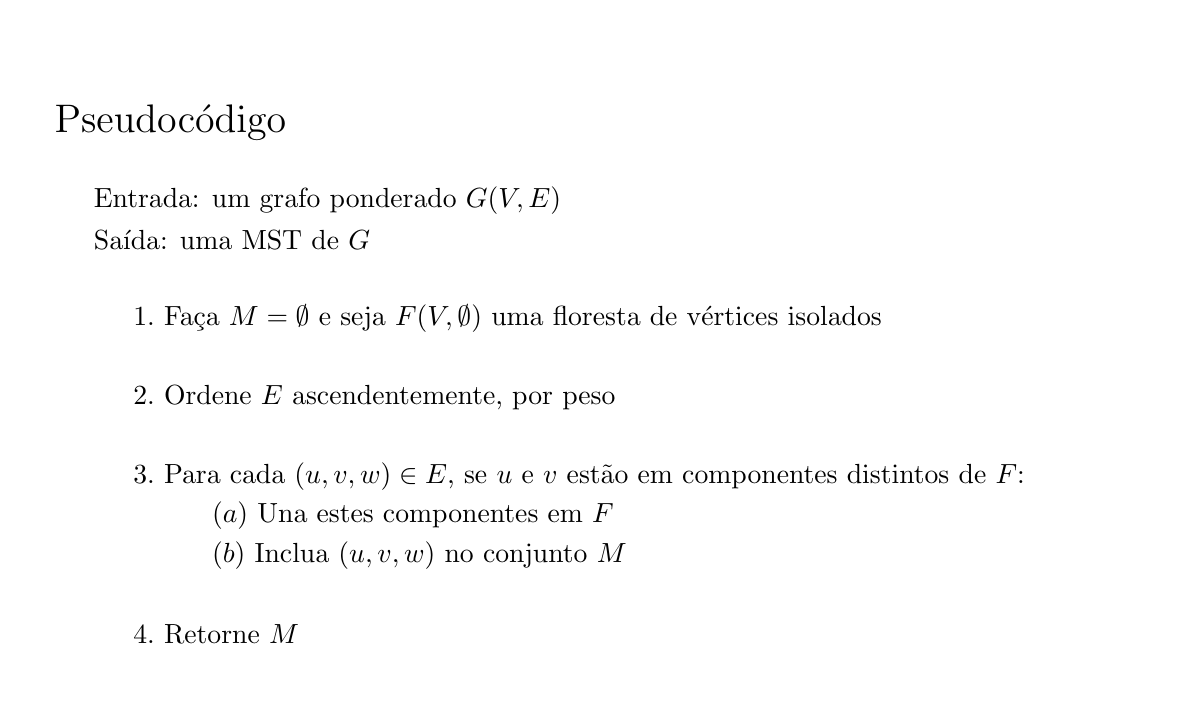
\begin{tikzpicture}
\node[draw,opacity=0] at (0, 0) {x};
\node[draw,opacity=0] at (14, 8) {x};

	\node[anchor=west] (title) at (0.0, 7.0) { \Large \bbbold{Pseudocódigo} };


	\node[anchor=west] (input) at (0.5, 6.0) { \bbemph{Entrada:} \bbtext{um grafo ponderado $G(V, E)$} };

	\node[anchor=west] (output) at (0.5, 5.5) { \bbemph{Saída:} \bbtext{uma MST de $G$} };

	\node[anchor=west] (step1) at (1.0, 4.5) { $1.$ \bbtext{Faça $M = \emptyset$ e seja $F(V, \emptyset)$ uma floresta de vértices isolados} };

	\node[anchor=west] (step2) at (1.0, 3.5) { $2.$ \bbtext{Ordene $E$ ascendentemente, por peso} };

	\node[anchor=west] (step3) at (1.0, 2.5) { $3.$ \bbtext{Para cada $(u, v, w)\in E$, se $u$ e $v$ estão em componentes distintos de $F$:} };

	\node[anchor=west] (step3a) at (2.0, 2.0) { $(a)$ \bbtext{Una estes componentes em $F$} };

	\node[anchor=west] (step3b) at (2.0, 1.5) { $(b)$ \bbtext{Inclua $(u, v, w)$ no conjunto $M$} };

	\node[anchor=west] (step4) at (1.0, 0.5) { $4.$ \bbtext{Retorne $M$} };


\end{tikzpicture}
\end{frame}
\begin{frame}[plain,t]
\begin{tikzpicture}
\node[draw,opacity=0] at (0, 0) {x};
\node[draw,opacity=0] at (14, 8) {x};

	\node[anchor=west] (x1) at (10.0, 6.0) { \bbtext{\tt 1 2 3} };

	\node[anchor=west] (x2) at (10.0, 5.5) { \bbtext{\tt 1 4 5} };

	\node[anchor=west] (x3) at (10.0, 5.0) { \bbtext{\tt 2 4 1} };

	\node[anchor=west] (x4) at (10.0, 4.5) { \bbtext{\tt 2 1 5} };

	\node[anchor=west] (x5) at (10.0, 4.0) { \bbtext{\tt 3 3 4} };

	\node[anchor=west] (x6) at (10.0, 3.5) { \bbtext{\tt 4 2 1} };

	\node[anchor=west] (x7) at (10.0, 3.0) { \bbtext{\tt 5 3 1} };

	\node[anchor=west] (x8) at (10.0, 2.5) { \bbtext{\tt 7 3 6} };

	\node[anchor=west] (x9) at (10.0, 2.0) { \bbtext{\tt 8 6 5} };

	\node[anchor=west] (E) at (10.4, 6.75) { \large $E$ };


	\node[very thick,draw,circle] (node1) at (6.0, 5.0) { \bbtext{1} };

	\node[very thick,draw,circle] (node2) at (4.0, 7.0) { \bbtext{2} };

	\node[very thick,draw,circle] (node3) at (2.0, 5.0) { \bbtext{3} };

	\node[very thick,draw,circle] (node4) at (6.0, 3.0) { \bbtext{4} };

	\node[very thick,draw,circle] (node5) at (4.0, 1.0) { \bbtext{5} };

	\node[very thick,draw,circle] (node6) at (2.0, 3.0) { \bbtext{6} };

\end{tikzpicture}
\end{frame}
\begin{frame}[plain,t]
\begin{tikzpicture}
\node[draw,opacity=0] at (0, 0) {x};
\node[draw,opacity=0] at (14, 8) {x};

	\node[anchor=west] (x1) at (10.0, 6.0) { \bbtext{\tt 1 2 3}\ \ \footnotesize{\textcolor{BBGreen}{\faCheck}} };

	\node[anchor=west] (x2) at (10.0, 5.5) { \bbtext{\tt 1 4 5} };

	\node[anchor=west] (x3) at (10.0, 5.0) { \bbtext{\tt 2 4 1} };

	\node[anchor=west] (x4) at (10.0, 4.5) { \bbtext{\tt 2 1 5} };

	\node[anchor=west] (x5) at (10.0, 4.0) { \bbtext{\tt 3 3 4} };

	\node[anchor=west] (x6) at (10.0, 3.5) { \bbtext{\tt 4 2 1} };

	\node[anchor=west] (x7) at (10.0, 3.0) { \bbtext{\tt 5 3 1} };

	\node[anchor=west] (x8) at (10.0, 2.5) { \bbtext{\tt 7 3 6} };

	\node[anchor=west] (x9) at (10.0, 2.0) { \bbtext{\tt 8 6 5} };

	\node[anchor=west] (E) at (10.4, 6.75) { \large $E$ };


	\node[very thick,draw,circle] (node1) at (6.0, 5.0) { \bbtext{1} };

	\node[very thick,draw,circle] (node2) at (4.0, 7.0) { \bbtext{2} };

	\node[very thick,draw,circle] (node3) at (2.0, 5.0) { \bbtext{3} };

	\node[very thick,draw,circle] (node4) at (6.0, 3.0) { \bbtext{4} };

	\node[very thick,draw,circle] (node5) at (4.0, 1.0) { \bbtext{5} };

	\node[very thick,draw,circle] (node6) at (2.0, 3.0) { \bbtext{6} };


	\draw[thick](node2) to node[above left] {\footnotesize \bbinfo{1}} (node3);


\end{tikzpicture}
\end{frame}
\begin{frame}[plain,t]
\begin{tikzpicture}
\node[draw,opacity=0] at (0, 0) {x};
\node[draw,opacity=0] at (14, 8) {x};

	\node[anchor=west] (x1) at (10.0, 6.0) { \bbtext{\tt 1 2 3}\ \ \footnotesize{\textcolor{BBGreen}{\faCheck}} };

	\node[anchor=west] (x2) at (10.0, 5.5) { \bbtext{\tt 1 4 5}\ \ \footnotesize{\textcolor{BBGreen}{\faCheck}} };

	\node[anchor=west] (x3) at (10.0, 5.0) { \bbtext{\tt 2 4 1} };

	\node[anchor=west] (x4) at (10.0, 4.5) { \bbtext{\tt 2 1 5} };

	\node[anchor=west] (x5) at (10.0, 4.0) { \bbtext{\tt 3 3 4} };

	\node[anchor=west] (x6) at (10.0, 3.5) { \bbtext{\tt 4 2 1} };

	\node[anchor=west] (x7) at (10.0, 3.0) { \bbtext{\tt 5 3 1} };

	\node[anchor=west] (x8) at (10.0, 2.5) { \bbtext{\tt 7 3 6} };

	\node[anchor=west] (x9) at (10.0, 2.0) { \bbtext{\tt 8 6 5} };

	\node[anchor=west] (E) at (10.4, 6.75) { \large $E$ };


	\node[very thick,draw,circle] (node1) at (6.0, 5.0) { \bbtext{1} };

	\node[very thick,draw,circle] (node2) at (4.0, 7.0) { \bbtext{2} };

	\node[very thick,draw,circle] (node3) at (2.0, 5.0) { \bbtext{3} };

	\node[very thick,draw,circle] (node4) at (6.0, 3.0) { \bbtext{4} };

	\node[very thick,draw,circle] (node5) at (4.0, 1.0) { \bbtext{5} };

	\node[very thick,draw,circle] (node6) at (2.0, 3.0) { \bbtext{6} };


	\draw[thick](node2) to node[above left] {\footnotesize \bbinfo{1}} (node3);



	\draw[thick](node4) to node[below right] {\footnotesize \bbinfo{1}} (node5);


\end{tikzpicture}
\end{frame}
\begin{frame}[plain,t]
\begin{tikzpicture}
\node[draw,opacity=0] at (0, 0) {x};
\node[draw,opacity=0] at (14, 8) {x};

	\node[anchor=west] (x1) at (10.0, 6.0) { \bbtext{\tt 1 2 3}\ \ \footnotesize{\textcolor{BBGreen}{\faCheck}} };

	\node[anchor=west] (x2) at (10.0, 5.5) { \bbtext{\tt 1 4 5}\ \ \footnotesize{\textcolor{BBGreen}{\faCheck}} };

	\node[anchor=west] (x3) at (10.0, 5.0) { \bbtext{\tt 2 4 1}\ \ \footnotesize{\textcolor{BBGreen}{\faCheck}} };

	\node[anchor=west] (x4) at (10.0, 4.5) { \bbtext{\tt 2 1 5} };

	\node[anchor=west] (x5) at (10.0, 4.0) { \bbtext{\tt 3 3 4} };

	\node[anchor=west] (x6) at (10.0, 3.5) { \bbtext{\tt 4 2 1} };

	\node[anchor=west] (x7) at (10.0, 3.0) { \bbtext{\tt 5 3 1} };

	\node[anchor=west] (x8) at (10.0, 2.5) { \bbtext{\tt 7 3 6} };

	\node[anchor=west] (x9) at (10.0, 2.0) { \bbtext{\tt 8 6 5} };

	\node[anchor=west] (E) at (10.4, 6.75) { \large $E$ };


	\node[very thick,draw,circle] (node1) at (6.0, 5.0) { \bbtext{1} };

	\node[very thick,draw,circle] (node2) at (4.0, 7.0) { \bbtext{2} };

	\node[very thick,draw,circle] (node3) at (2.0, 5.0) { \bbtext{3} };

	\node[very thick,draw,circle] (node4) at (6.0, 3.0) { \bbtext{4} };

	\node[very thick,draw,circle] (node5) at (4.0, 1.0) { \bbtext{5} };

	\node[very thick,draw,circle] (node6) at (2.0, 3.0) { \bbtext{6} };


	\draw[thick](node2) to node[above left] {\footnotesize \bbinfo{1}} (node3);



	\draw[thick](node4) to node[below right] {\footnotesize \bbinfo{1}} (node5);



	\draw[thick](node1) to node[right] {\footnotesize \bbinfo{2}} (node4);


\end{tikzpicture}
\end{frame}
\begin{frame}[plain,t]
\begin{tikzpicture}
\node[draw,opacity=0] at (0, 0) {x};
\node[draw,opacity=0] at (14, 8) {x};

	\node[anchor=west] (x1) at (10.0, 6.0) { \bbtext{\tt 1 2 3}\ \ \footnotesize{\textcolor{BBGreen}{\faCheck}} };

	\node[anchor=west] (x2) at (10.0, 5.5) { \bbtext{\tt 1 4 5}\ \ \footnotesize{\textcolor{BBGreen}{\faCheck}} };

	\node[anchor=west] (x3) at (10.0, 5.0) { \bbtext{\tt 2 4 1}\ \ \footnotesize{\textcolor{BBGreen}{\faCheck}} };

	\node[anchor=west] (x4) at (10.0, 4.5) { \bbtext{\tt 2 1 5}\ \ \footnotesize{\textcolor{BBRed}{\faClose}} };

	\node[anchor=west] (x5) at (10.0, 4.0) { \bbtext{\tt 3 3 4} };

	\node[anchor=west] (x6) at (10.0, 3.5) { \bbtext{\tt 4 2 1} };

	\node[anchor=west] (x7) at (10.0, 3.0) { \bbtext{\tt 5 3 1} };

	\node[anchor=west] (x8) at (10.0, 2.5) { \bbtext{\tt 7 3 6} };

	\node[anchor=west] (x9) at (10.0, 2.0) { \bbtext{\tt 8 6 5} };

	\node[anchor=west] (E) at (10.4, 6.75) { \large $E$ };


	\node[very thick,draw,circle] (node1) at (6.0, 5.0) { \bbtext{1} };

	\node[very thick,draw,circle] (node2) at (4.0, 7.0) { \bbtext{2} };

	\node[very thick,draw,circle] (node3) at (2.0, 5.0) { \bbtext{3} };

	\node[very thick,draw,circle] (node4) at (6.0, 3.0) { \bbtext{4} };

	\node[very thick,draw,circle] (node5) at (4.0, 1.0) { \bbtext{5} };

	\node[very thick,draw,circle] (node6) at (2.0, 3.0) { \bbtext{6} };


	\draw[thick](node2) to node[above left] {\footnotesize \bbinfo{1}} (node3);



	\draw[thick](node4) to node[below right] {\footnotesize \bbinfo{1}} (node5);



	\draw[thick](node1) to node[right] {\footnotesize \bbinfo{2}} (node4);




\end{tikzpicture}
\end{frame}
\begin{frame}[plain,t]
\begin{tikzpicture}
\node[draw,opacity=0] at (0, 0) {x};
\node[draw,opacity=0] at (14, 8) {x};

	\node[anchor=west] (x1) at (10.0, 6.0) { \bbtext{\tt 1 2 3}\ \ \footnotesize{\textcolor{BBGreen}{\faCheck}} };

	\node[anchor=west] (x2) at (10.0, 5.5) { \bbtext{\tt 1 4 5}\ \ \footnotesize{\textcolor{BBGreen}{\faCheck}} };

	\node[anchor=west] (x3) at (10.0, 5.0) { \bbtext{\tt 2 4 1}\ \ \footnotesize{\textcolor{BBGreen}{\faCheck}} };

	\node[anchor=west] (x4) at (10.0, 4.5) { \bbtext{\tt 2 1 5}\ \ \footnotesize{\textcolor{BBRed}{\faClose}} };

	\node[anchor=west] (x5) at (10.0, 4.0) { \bbtext{\tt 3 3 4}\ \ \footnotesize{\textcolor{BBGreen}{\faCheck}} };

	\node[anchor=west] (x6) at (10.0, 3.5) { \bbtext{\tt 4 2 1} };

	\node[anchor=west] (x7) at (10.0, 3.0) { \bbtext{\tt 5 3 1} };

	\node[anchor=west] (x8) at (10.0, 2.5) { \bbtext{\tt 7 3 6} };

	\node[anchor=west] (x9) at (10.0, 2.0) { \bbtext{\tt 8 6 5} };

	\node[anchor=west] (E) at (10.4, 6.75) { \large $E$ };


	\node[very thick,draw,circle] (node1) at (6.0, 5.0) { \bbtext{1} };

	\node[very thick,draw,circle] (node2) at (4.0, 7.0) { \bbtext{2} };

	\node[very thick,draw,circle] (node3) at (2.0, 5.0) { \bbtext{3} };

	\node[very thick,draw,circle] (node4) at (6.0, 3.0) { \bbtext{4} };

	\node[very thick,draw,circle] (node5) at (4.0, 1.0) { \bbtext{5} };

	\node[very thick,draw,circle] (node6) at (2.0, 3.0) { \bbtext{6} };


	\draw[thick](node2) to node[above left] {\footnotesize \bbinfo{1}} (node3);



	\draw[thick](node4) to node[below right] {\footnotesize \bbinfo{1}} (node5);



	\draw[thick](node1) to node[right] {\footnotesize \bbinfo{2}} (node4);





	\draw[thick](node3) to node[above] {\footnotesize \bbinfo{3}} (node4);


\end{tikzpicture}
\end{frame}
\begin{frame}[plain,t]
\begin{tikzpicture}
\node[draw,opacity=0] at (0, 0) {x};
\node[draw,opacity=0] at (14, 8) {x};

	\node[anchor=west] (x1) at (10.0, 6.0) { \bbtext{\tt 1 2 3}\ \ \footnotesize{\textcolor{BBGreen}{\faCheck}} };

	\node[anchor=west] (x2) at (10.0, 5.5) { \bbtext{\tt 1 4 5}\ \ \footnotesize{\textcolor{BBGreen}{\faCheck}} };

	\node[anchor=west] (x3) at (10.0, 5.0) { \bbtext{\tt 2 4 1}\ \ \footnotesize{\textcolor{BBGreen}{\faCheck}} };

	\node[anchor=west] (x4) at (10.0, 4.5) { \bbtext{\tt 2 1 5}\ \ \footnotesize{\textcolor{BBRed}{\faClose}} };

	\node[anchor=west] (x5) at (10.0, 4.0) { \bbtext{\tt 3 3 4}\ \ \footnotesize{\textcolor{BBGreen}{\faCheck}} };

	\node[anchor=west] (x6) at (10.0, 3.5) { \bbtext{\tt 4 2 1}\ \ \footnotesize{\textcolor{BBRed}{\faClose}} };

	\node[anchor=west] (x7) at (10.0, 3.0) { \bbtext{\tt 5 3 1} };

	\node[anchor=west] (x8) at (10.0, 2.5) { \bbtext{\tt 7 3 6} };

	\node[anchor=west] (x9) at (10.0, 2.0) { \bbtext{\tt 8 6 5} };

	\node[anchor=west] (E) at (10.4, 6.75) { \large $E$ };


	\node[very thick,draw,circle] (node1) at (6.0, 5.0) { \bbtext{1} };

	\node[very thick,draw,circle] (node2) at (4.0, 7.0) { \bbtext{2} };

	\node[very thick,draw,circle] (node3) at (2.0, 5.0) { \bbtext{3} };

	\node[very thick,draw,circle] (node4) at (6.0, 3.0) { \bbtext{4} };

	\node[very thick,draw,circle] (node5) at (4.0, 1.0) { \bbtext{5} };

	\node[very thick,draw,circle] (node6) at (2.0, 3.0) { \bbtext{6} };


	\draw[thick](node2) to node[above left] {\footnotesize \bbinfo{1}} (node3);



	\draw[thick](node4) to node[below right] {\footnotesize \bbinfo{1}} (node5);



	\draw[thick](node1) to node[right] {\footnotesize \bbinfo{2}} (node4);





	\draw[thick](node3) to node[above] {\footnotesize \bbinfo{3}} (node4);




\end{tikzpicture}
\end{frame}
\begin{frame}[plain,t]
\begin{tikzpicture}
\node[draw,opacity=0] at (0, 0) {x};
\node[draw,opacity=0] at (14, 8) {x};

	\node[anchor=west] (x1) at (10.0, 6.0) { \bbtext{\tt 1 2 3}\ \ \footnotesize{\textcolor{BBGreen}{\faCheck}} };

	\node[anchor=west] (x2) at (10.0, 5.5) { \bbtext{\tt 1 4 5}\ \ \footnotesize{\textcolor{BBGreen}{\faCheck}} };

	\node[anchor=west] (x3) at (10.0, 5.0) { \bbtext{\tt 2 4 1}\ \ \footnotesize{\textcolor{BBGreen}{\faCheck}} };

	\node[anchor=west] (x4) at (10.0, 4.5) { \bbtext{\tt 2 1 5}\ \ \footnotesize{\textcolor{BBRed}{\faClose}} };

	\node[anchor=west] (x5) at (10.0, 4.0) { \bbtext{\tt 3 3 4}\ \ \footnotesize{\textcolor{BBGreen}{\faCheck}} };

	\node[anchor=west] (x6) at (10.0, 3.5) { \bbtext{\tt 4 2 1}\ \ \footnotesize{\textcolor{BBRed}{\faClose}} };

	\node[anchor=west] (x7) at (10.0, 3.0) { \bbtext{\tt 5 3 1}\ \ \footnotesize{\textcolor{BBRed}{\faClose}} };

	\node[anchor=west] (x8) at (10.0, 2.5) { \bbtext{\tt 7 3 6} };

	\node[anchor=west] (x9) at (10.0, 2.0) { \bbtext{\tt 8 6 5} };

	\node[anchor=west] (E) at (10.4, 6.75) { \large $E$ };


	\node[very thick,draw,circle] (node1) at (6.0, 5.0) { \bbtext{1} };

	\node[very thick,draw,circle] (node2) at (4.0, 7.0) { \bbtext{2} };

	\node[very thick,draw,circle] (node3) at (2.0, 5.0) { \bbtext{3} };

	\node[very thick,draw,circle] (node4) at (6.0, 3.0) { \bbtext{4} };

	\node[very thick,draw,circle] (node5) at (4.0, 1.0) { \bbtext{5} };

	\node[very thick,draw,circle] (node6) at (2.0, 3.0) { \bbtext{6} };


	\draw[thick](node2) to node[above left] {\footnotesize \bbinfo{1}} (node3);



	\draw[thick](node4) to node[below right] {\footnotesize \bbinfo{1}} (node5);



	\draw[thick](node1) to node[right] {\footnotesize \bbinfo{2}} (node4);





	\draw[thick](node3) to node[above] {\footnotesize \bbinfo{3}} (node4);






\end{tikzpicture}
\end{frame}
\begin{frame}[plain,t]
\begin{tikzpicture}
\node[draw,opacity=0] at (0, 0) {x};
\node[draw,opacity=0] at (14, 8) {x};

	\node[anchor=west] (x1) at (10.0, 6.0) { \bbtext{\tt 1 2 3}\ \ \footnotesize{\textcolor{BBGreen}{\faCheck}} };

	\node[anchor=west] (x2) at (10.0, 5.5) { \bbtext{\tt 1 4 5}\ \ \footnotesize{\textcolor{BBGreen}{\faCheck}} };

	\node[anchor=west] (x3) at (10.0, 5.0) { \bbtext{\tt 2 4 1}\ \ \footnotesize{\textcolor{BBGreen}{\faCheck}} };

	\node[anchor=west] (x4) at (10.0, 4.5) { \bbtext{\tt 2 1 5}\ \ \footnotesize{\textcolor{BBRed}{\faClose}} };

	\node[anchor=west] (x5) at (10.0, 4.0) { \bbtext{\tt 3 3 4}\ \ \footnotesize{\textcolor{BBGreen}{\faCheck}} };

	\node[anchor=west] (x6) at (10.0, 3.5) { \bbtext{\tt 4 2 1}\ \ \footnotesize{\textcolor{BBRed}{\faClose}} };

	\node[anchor=west] (x7) at (10.0, 3.0) { \bbtext{\tt 5 3 1}\ \ \footnotesize{\textcolor{BBRed}{\faClose}} };

	\node[anchor=west] (x8) at (10.0, 2.5) { \bbtext{\tt 7 3 6}\ \ \footnotesize{\textcolor{BBGreen}{\faCheck}} };

	\node[anchor=west] (x9) at (10.0, 2.0) { \bbtext{\tt 8 6 5} };

	\node[anchor=west] (E) at (10.4, 6.75) { \large $E$ };


	\node[very thick,draw,circle] (node1) at (6.0, 5.0) { \bbtext{1} };

	\node[very thick,draw,circle] (node2) at (4.0, 7.0) { \bbtext{2} };

	\node[very thick,draw,circle] (node3) at (2.0, 5.0) { \bbtext{3} };

	\node[very thick,draw,circle] (node4) at (6.0, 3.0) { \bbtext{4} };

	\node[very thick,draw,circle] (node5) at (4.0, 1.0) { \bbtext{5} };

	\node[very thick,draw,circle] (node6) at (2.0, 3.0) { \bbtext{6} };


	\draw[thick](node2) to node[above left] {\footnotesize \bbinfo{1}} (node3);



	\draw[thick](node4) to node[below right] {\footnotesize \bbinfo{1}} (node5);



	\draw[thick](node1) to node[right] {\footnotesize \bbinfo{2}} (node4);





	\draw[thick](node3) to node[above] {\footnotesize \bbinfo{3}} (node4);







	\draw[thick](node3) to node[below left] {\footnotesize \bbinfo{7}} (node6);


\end{tikzpicture}
\end{frame}
\begin{frame}[plain,t]
\begin{tikzpicture}
\node[draw,opacity=0] at (0, 0) {x};
\node[draw,opacity=0] at (14, 8) {x};

	\node[anchor=west] (x1) at (10.0, 6.0) { \bbtext{\tt 1 2 3}\ \ \footnotesize{\textcolor{BBGreen}{\faCheck}} };

	\node[anchor=west] (x2) at (10.0, 5.5) { \bbtext{\tt 1 4 5}\ \ \footnotesize{\textcolor{BBGreen}{\faCheck}} };

	\node[anchor=west] (x3) at (10.0, 5.0) { \bbtext{\tt 2 4 1}\ \ \footnotesize{\textcolor{BBGreen}{\faCheck}} };

	\node[anchor=west] (x4) at (10.0, 4.5) { \bbtext{\tt 2 1 5}\ \ \footnotesize{\textcolor{BBRed}{\faClose}} };

	\node[anchor=west] (x5) at (10.0, 4.0) { \bbtext{\tt 3 3 4}\ \ \footnotesize{\textcolor{BBGreen}{\faCheck}} };

	\node[anchor=west] (x6) at (10.0, 3.5) { \bbtext{\tt 4 2 1}\ \ \footnotesize{\textcolor{BBRed}{\faClose}} };

	\node[anchor=west] (x7) at (10.0, 3.0) { \bbtext{\tt 5 3 1}\ \ \footnotesize{\textcolor{BBRed}{\faClose}} };

	\node[anchor=west] (x8) at (10.0, 2.5) { \bbtext{\tt 7 3 6}\ \ \footnotesize{\textcolor{BBGreen}{\faCheck}} };

	\node[anchor=west] (x9) at (10.0, 2.0) { \bbtext{\tt 8 6 5}\ \ \footnotesize{\textcolor{BBRed}{\faClose}} };

	\node[anchor=west] (E) at (10.4, 6.75) { \large $E$ };


	\node[very thick,draw,circle] (node1) at (6.0, 5.0) { \bbtext{1} };

	\node[very thick,draw,circle] (node2) at (4.0, 7.0) { \bbtext{2} };

	\node[very thick,draw,circle] (node3) at (2.0, 5.0) { \bbtext{3} };

	\node[very thick,draw,circle] (node4) at (6.0, 3.0) { \bbtext{4} };

	\node[very thick,draw,circle] (node5) at (4.0, 1.0) { \bbtext{5} };

	\node[very thick,draw,circle] (node6) at (2.0, 3.0) { \bbtext{6} };


	\draw[thick](node2) to node[above left] {\footnotesize \bbinfo{1}} (node3);



	\draw[thick](node4) to node[below right] {\footnotesize \bbinfo{1}} (node5);



	\draw[thick](node1) to node[right] {\footnotesize \bbinfo{2}} (node4);





	\draw[thick](node3) to node[above] {\footnotesize \bbinfo{3}} (node4);







	\draw[thick](node3) to node[below left] {\footnotesize \bbinfo{7}} (node6);




\end{tikzpicture}
\end{frame}
\begin{frame}[plain,t]

\inputsnippet{cpp}{46}{63}{codes/kruskal.cpp}

\end{frame}
\begin{frame}[plain,t]
\begin{tikzpicture}
\node[draw,opacity=0] at (0, 0) {x};
\node[draw,opacity=0] at (14, 8) {x};

	\node[anchor=west] (title) at (0.0, 6.0) { \Large \bbbold{Problemas sugeridos} };

	\node[anchor=west] (a) at (1.0, 5.0) { $1.$ \bbtext{Codeforces Round \#179 (Div. 1) -- Problem B: Greg and Graph} };

	\node[anchor=west] (b) at (1.0, 4.0) { $2.$ \bbtext{LightOJ -- Travel Company} };

	\node[anchor=west] (c) at (1.0, 3.0) { $3.$ \bbtext{OJ 104 -- Arbitrage} };

	\node[anchor=west] (d) at (1.0, 2.0) { $4.$ \bbtext{OJ 10171 -- Meeting Prof. Miguel...} };

\end{tikzpicture}
\end{frame}
\begin{frame}[plain,t]
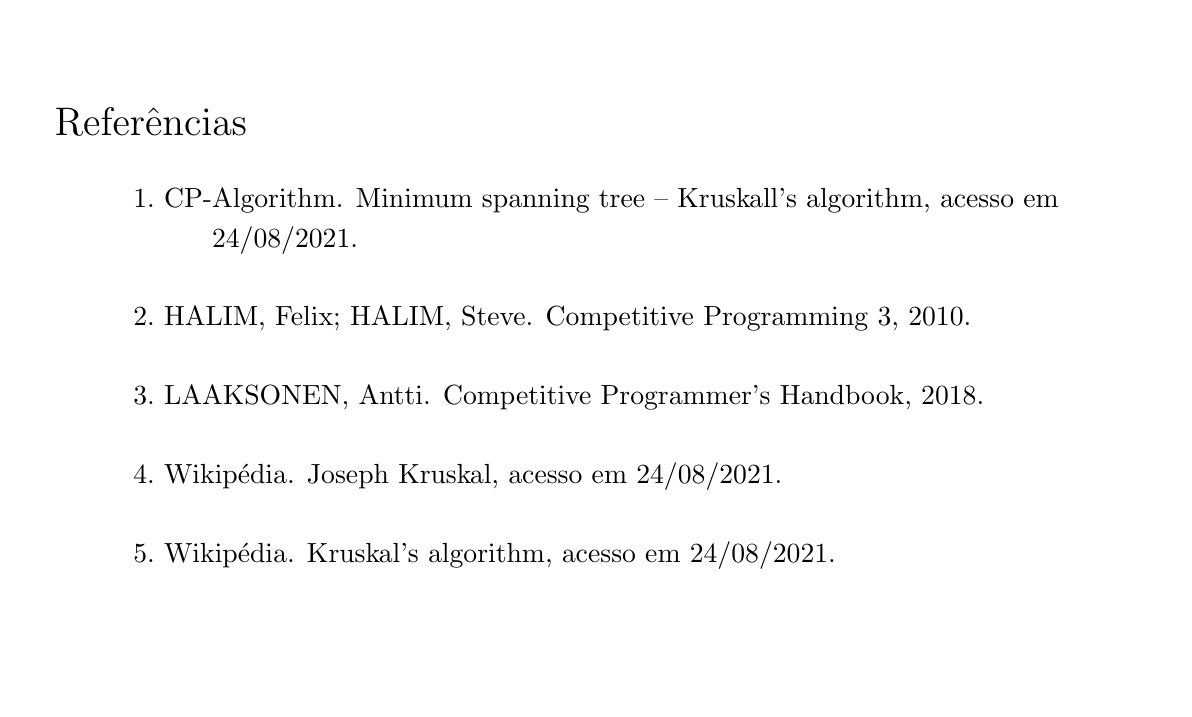
\begin{tikzpicture}
\node[draw,opacity=0] at (0, 0) {x};
\node[draw,opacity=0] at (14, 8) {x};

	\node[anchor=west] (title) at (0.0, 7.0) { \Large \bbbold{Referências} };

	\node[anchor=west] (a) at (1.0, 6.0) { $1.$ \bbtext{\bbbold{CP-Algorithm}. \bbenglish{Minimum spanning tree -- Kruskall's algorithm}, acesso em} };

	\node[anchor=west] (a1) at (2.0, 5.5) { \bbtext{24/08/2021.} };

	\node[anchor=west] (b) at (1.0, 4.5) { $2.$ \bbbold{HALIM}, \bbtext{Felix}; \bbbold{HALIM}, \bbtext{Steve}. \bbenglish{Competitive Programming 3,} \bbtext{2010.} };

	\node[anchor=west] (c) at (1.0, 3.5) { $3.$ \bbbold{LAAKSONEN}, \bbtext{Antti}. \bbenglish{Competitive Programmer's Handbook,} \bbtext{2018.} };

	\node[anchor=west] (d) at (1.0, 2.5) { $4.$ \bbbold{Wikipédia}. \bbenglish{Joseph Kruskal,} \bbtext{acesso em 24/08/2021.} };

	\node[anchor=west] (e) at (1.0, 1.5) { $5.$ \bbbold{Wikipédia}. \bbenglish{Kruskal's algorithm,} \bbtext{acesso em 24/08/2021.} };


\end{tikzpicture}
\end{frame}
\end{document}
